
%(BEGIN_QUESTION)
% Copyright 2007, Tony R. Kuphaldt, released under the Creative Commons Attribution License (v 1.0)
% This means you may do almost anything with this work of mine, so long as you give me proper credit

Is this network a EIA/TIA-422 or a EIA/TIA-485?  Is it possible to tell from this diagram, and if so, how?

$$\includegraphics[width=15.5cm]{i02197x01.eps}$$

\underbar{file i02197}
%(END_QUESTION)





%(BEGIN_ANSWER)

This must be a EIA/TIA-485 network, because there is more than one driver connected to the same pair of lines.  In other words, this is a multi{\it point} system, rather than a multi{\it drop} system where there is only one driver (transmitter) and multiple listeners (receivers).

%(END_ANSWER)





%(BEGIN_NOTES)

According to Texas Instrument's document {\it 422 and 485 Standards Overview and System Configurations}, the EIA/TIA-422 standard is a simplex multidrop system, allowing for one transmitter (driver) and a maximum of ten receivers.  The EIA/TIA-485 standard, on the other hand, is a half-duplex multipoint system.  Multiple transmitters (drivers) are allowed on a bus, but only one may transmit at a time.

%INDEX% Networking, multidrop: EIA/TIA-422
%INDEX% Networking, multidrop: EIA/TIA-485
%INDEX% Networking, multipoint: EIA/TIA-485

%(END_NOTES)


